\documentclass[aspectratio=169,11pt]{beamer}
\usepackage[T1]{fontenc}
\usepackage{lmodern}
\usepackage{amsmath,amssymb,booktabs,listings}
\usetheme{Madrid}
\usecolortheme{dolphin}
\setbeamertemplate{blocks}[rounded][shadow=false]
\definecolor{Navy}{HTML}{15345C}
\definecolor{Teal}{HTML}{2266B3}
\definecolor{Coral}{HTML}{D6603C}
\definecolor{Mist}{HTML}{EFF5FC}
\setbeamercolor{normal text}{fg=Navy,bg=white}
\setbeamercolor{structure}{fg=Teal}
\setbeamercolor{frametitle}{fg=white,bg=Navy}
\setbeamercolor{title}{fg=white,bg=Navy}
\setbeamercolor{subtitle}{fg=white}
\setbeamercolor{alerted text}{fg=Teal}
\setbeamercolor{palette primary}{fg=white,bg=Teal}
\setbeamercolor{palette secondary}{fg=white,bg=Navy}
\setbeamercolor{palette tertiary}{fg=white,bg=Navy}
\setbeamercolor{block title}{fg=white,bg=Teal}
\setbeamercolor{block body}{fg=Navy,bg=Mist}
\setbeamerfont{title}{size=\Huge,series=\bfseries}
\setbeamerfont{frametitle}{size=\Large,series=\bfseries}
\setbeamertemplate{navigation symbols}{}
\setbeamertemplate{itemize items}[circle]
\setbeamersize{text margin left=9mm,text margin right=9mm}
\setbeamertemplate{headline}{}
\setbeamertemplate{footline}{%
 \leavevmode\hbox{%
 \begin{beamercolorbox}[wd=.84\paperwidth,ht=2.8ex,dp=1.2ex,leftskip=9mm]{palette secondary}%
 \scriptsize DRP\enspace\textbar\enspace GAN Learning
 \end{beamercolorbox}%
 \begin{beamercolorbox}[wd=.16\paperwidth,ht=2.8ex,dp=1.2ex,center]{palette primary}%
 \scriptsize\insertframenumber\,/\,\inserttotalframenumber
 \end{beamercolorbox}}}
\lstset{language=Python,basicstyle=\ttfamily\small,keywordstyle=\color{Teal}\bfseries,
 stringstyle=\color{Coral},showstringspaces=false,columns=fullflexible,keepspaces=true,
 frame=none,backgroundcolor=\color{Mist},xleftmargin=2mm,xrightmargin=2mm,
 aboveskip=3mm,belowskip=3mm,breaklines=false}
\newcommand{\ganref}{\vfill{\tiny\color{gray}Goodfellow et al. (2014), \href{https://arxiv.org/abs/1406.2661}{Generative Adversarial Nets}, Section 3.}}
\title{Generative adversarial\\networks}
\subtitle{A first example: learning to generate numbers}
\author{\texorpdfstring{Directed Reading Program\\Florida State University}{Directed Reading Program, Florida State University}}
\date{}
\begin{document}

\begin{frame}
\titlepage
\vspace{-5mm}
\centering\textcolor{Teal}{Data \quad Two networks \quad Two losses \quad Generation}
\end{frame}

\begin{frame}{Learning a function and learning a distribution}
\begin{center}
\begin{tabular}{p{.22\textwidth}p{.31\textwidth}p{.31\textwidth}}
\toprule
& Previous lesson & This lesson\\\midrule
Input & A chosen value $x$ & Random noise $z$\\[3mm]
Output & A prediction $f_\theta(x)$ & A generated sample $G_\theta(z)$\\[3mm]
Learning signal & A target $\sin(x)$ & A learned discriminator\\[3mm]
Evaluation & Error at new inputs & Distribution of new samples\\\bottomrule
\end{tabular}
\end{center}
\vspace{4mm}
\large A generated sample has no paired correct answer.
\end{frame}

\begin{frame}[fragile]{1. Real data: a bell-shaped distribution}
\begin{columns}[c]
\begin{column}{.44\textwidth}
\[X\sim\mathcal N(2,0.5^2)\]
\begin{lstlisting}[basicstyle=\ttfamily\footnotesize]
torch.manual_seed(7)
x_train = 2 + 0.5 * torch.randn(
    2048, 1
)
\end{lstlisting}
\small
2,048 samples, each a single number.\\[3mm]
Mean $2$, standard deviation $0.5$.\\[3mm]
We know the distribution so we can check the result.
\end{column}
\begin{column}{.55\textwidth}
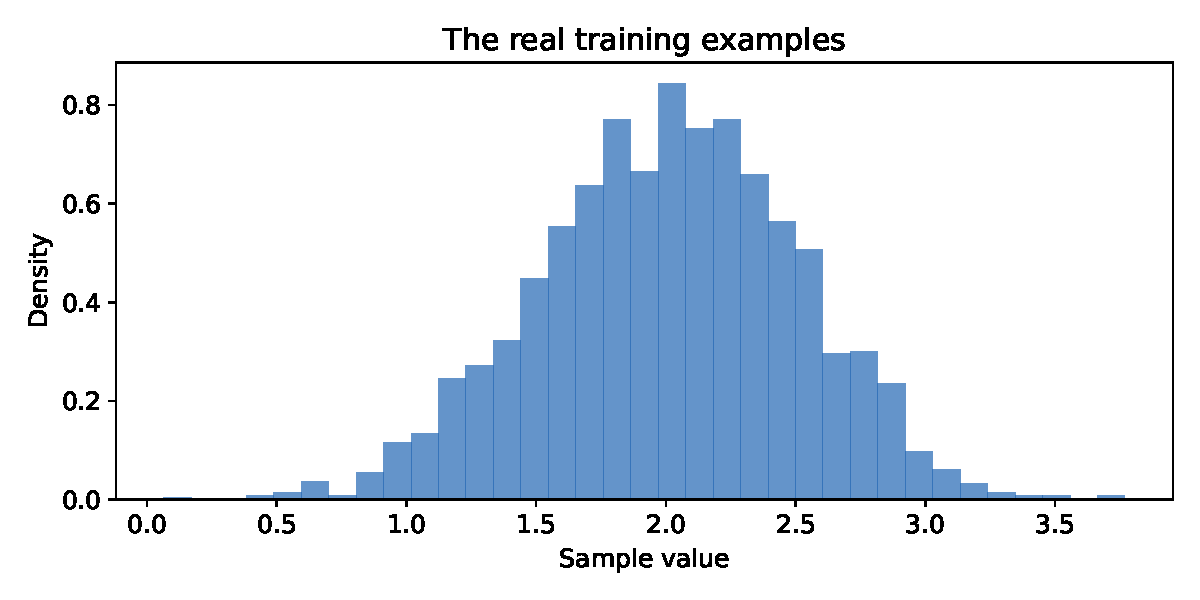
\includegraphics[width=\linewidth]{figures/training_data.pdf}
\end{column}
\end{columns}
\vspace{3mm}
\small Direct sampling already works here. The GAN is a teaching example.
\end{frame}

\begin{frame}{Two networks with different jobs}
\begin{columns}[t]
\begin{column}{.47\textwidth}
\textcolor{Teal}{\large Generator $G_\theta$}
\[z\sim\mathcal N(0,1),\quad x_{\mathrm{fake}}=G_\theta(z)\]
Transforms noise into candidate samples.\\[4mm]
Learns to make the discriminator assign a high real-data probability.
\end{column}
\begin{column}{.47\textwidth}
\textcolor{Teal}{\large Discriminator $D_\phi$}
\[s=D_\phi(x),\quad d_\phi(x)=\sigma(s)\]
Receives real and generated samples.\\[4mm]
Learns to assign probability near 1 to real data and near 0 to generated data.
\end{column}
\end{columns}
\vspace{7mm}
Each has 49 parameters. We train the two parameter sets separately.
\ganref
\end{frame}

\begin{frame}[fragile]{2. The generator architecture}
\begin{columns}[c]
\begin{column}{.48\textwidth}
\begin{lstlisting}
G = nn.Sequential(
    nn.Linear(1, 16),
    nn.Tanh(),
    nn.Linear(16, 1)
)
\end{lstlisting}
\end{column}
\begin{column}{.47\textwidth}
\[G_\theta(z)=c+\sum_{j=1}^{16}v_j\tanh(w_jz+b_j)\]
\small
Input: one random number.\\[3mm]
Hidden layer: 16 nonlinear responses.\\[3mm]
Output: one generated number.
\end{column}
\end{columns}
\vspace{6mm}
The same architecture as the sine example, with a different training task.\\[3mm]
New noise gives new inputs. The same noise and parameters give the same output.
\end{frame}

\begin{frame}[fragile]{The discriminator returns a logit}
\begin{columns}[c]
\begin{column}{.47\textwidth}
\begin{lstlisting}
D = nn.Sequential(
    nn.Linear(1, 16),
    nn.Tanh(),
    nn.Linear(16, 1)
)
\end{lstlisting}
\end{column}
\begin{column}{.48\textwidth}
\[s=D_\phi(x)\in\mathbb R\]
\[d_\phi(x)=\sigma(s)=\frac{1}{1+e^{-s}}\]
\small
The logit $s$ is unrestricted. Its sigmoid is between 0 and 1.
\end{column}
\end{columns}
\vspace{5mm}
\texttt{BCEWithLogitsLoss} applies sigmoid internally for stable computation.\\[3mm]
We pass the raw logits into the loss.
\vfill{\tiny\color{gray}PyTorch: \href{https://docs.pytorch.org/docs/stable/generated/torch.nn.BCEWithLogitsLoss.html}{BCEWithLogitsLoss}.}
\end{frame}

\begin{frame}[fragile]{3. Binary cross-entropy}
For a logit $s$ and a label $t\in\{0,1\}$,
\[\ell(s,t)=-t\log\sigma(s)-(1-t)\log(1-\sigma(s)).\]
\begin{lstlisting}
bce = nn.BCEWithLogitsLoss()
\end{lstlisting}
\begin{center}
\begin{tabular}{lcc}
\toprule
Desired label & Predicted real probability & Loss\\\midrule
$t=1$ & $0.9$ & $-\log(0.9)\approx0.105$\\[2mm]
$t=1$ & $0.1$ & $-\log(0.1)\approx2.303$\\\bottomrule
\end{tabular}
\end{center}
\vspace{3mm}
Confident predictions of the wrong label incur a larger loss.
\end{frame}

\begin{frame}{The discriminator learns real versus generated}
\large
\[L_D=\frac1m\sum_i\ell(D_\phi(x_i),1)
+\frac1m\sum_i\ell(D_\phi(G_\theta(z_i)),0)\]
\normalsize
\begin{itemize}\setlength\itemsep{4mm}
\item Real training samples have label 1.
\item Generated samples have label 0.
\item This update changes only the discriminator parameters $\phi$.
\end{itemize}
\vspace{5mm}
The two terms are batch means, added together. This scaling matters when reading the loss plot.
\ganref
\end{frame}

\begin{frame}{The generator learns through the discriminator}
\large
\[L_G=\frac1m\sum_i\ell(D_\phi(G_\theta(z_i)),1)
=-\frac1m\sum_i\log d_\phi(G_\theta(z_i))\]
\normalsize
\begin{itemize}\setlength\itemsep{4mm}
\item The desired label is 1: the generator wants its samples classified as real.
\item This update changes only the generator parameters $\theta$.
\item The discriminator supplies a differentiable learning signal.
\end{itemize}
\vspace{3mm}
We use the \alert{non-saturating} generator objective, rather than the original minimax generator objective.
\ganref
\end{frame}

\begin{frame}[fragile]{Separate optimizers for separate parameter sets}
\begin{lstlisting}
opt_g = torch.optim.Adam(
    G.parameters(), lr=0.001, betas=(0.5, 0.999)
)
opt_d = torch.optim.Adam(
    D.parameters(), lr=0.001, betas=(0.5, 0.999)
)
\end{lstlisting}
\vspace{3mm}
Adam scales updates using running averages of gradients and squared gradients.\\[3mm]
The learning rate and \texttt{betas} are settings we choose before training.\\[3mm]
Each iteration has one discriminator update and one generator update.
\end{frame}

\begin{frame}[fragile]{4. Training: the discriminator step}
\begin{lstlisting}[basicstyle=\ttfamily\footnotesize]
d_history, g_history = [], []
for step in range(6000):
    real = x_train[torch.randint(len(x_train), (128,))]
    fake = G(torch.randn(128, 1))

    D.requires_grad_(True)
    opt_d.zero_grad()
    d_loss = bce(D(real), torch.ones(128, 1))
    d_loss = d_loss + bce(D(fake.detach()), torch.zeros(128, 1))
    d_loss.backward()
    opt_d.step()
\end{lstlisting}
\vspace{2mm}
\texttt{detach()} stops this backward pass at the generated samples.\\[2mm]
Real batches sample the training set with replacement. These are iterations, not full-data epochs.
\end{frame}

\begin{frame}[fragile]{Training: the generator step}
\small Continuation inside the same loop:
\begin{lstlisting}[basicstyle=\ttfamily\footnotesize]
    D.requires_grad_(False)
    opt_g.zero_grad()
    fake = G(torch.randn(128, 1))
    g_loss = bce(D(fake), torch.ones(128, 1))
    g_loss.backward()
    opt_g.step()

    d_history.append(d_loss.item())
    g_history.append(g_loss.item())
\end{lstlisting}
\vspace{2mm}
Freeze the discriminator parameters, but keep derivatives through its input.\\[2mm]
There is no \texttt{detach()} here: the gradient must reach the generator.
\end{frame}

\begin{frame}{How the gradient reaches the generator}
For one generated sample, let $s=D_\phi(G_\theta(z))$ and $d=\sigma(s)$.
\vspace{3mm}
\large
\[\nabla_\theta\ell(s,1)=
\underbrace{(d-1)}_{\text{loss derivative}}
\underbrace{D_\phi'(G_\theta(z))}_{\text{discriminator slope}}
\underbrace{\nabla_\theta G_\theta(z)}_{\text{generator derivative}}.\]
\normalsize
\vspace{6mm}
\begin{itemize}\setlength\itemsep{4mm}
\item Freezing $\phi$ keeps the discriminator parameters fixed for this update.
\item The slope with respect to its input still guides the generator.
\item \texttt{no\_grad()} would break the learning calculation here.
\end{itemize}
\end{frame}

\begin{frame}{GAN losses do not need to fall together}
\begin{center}
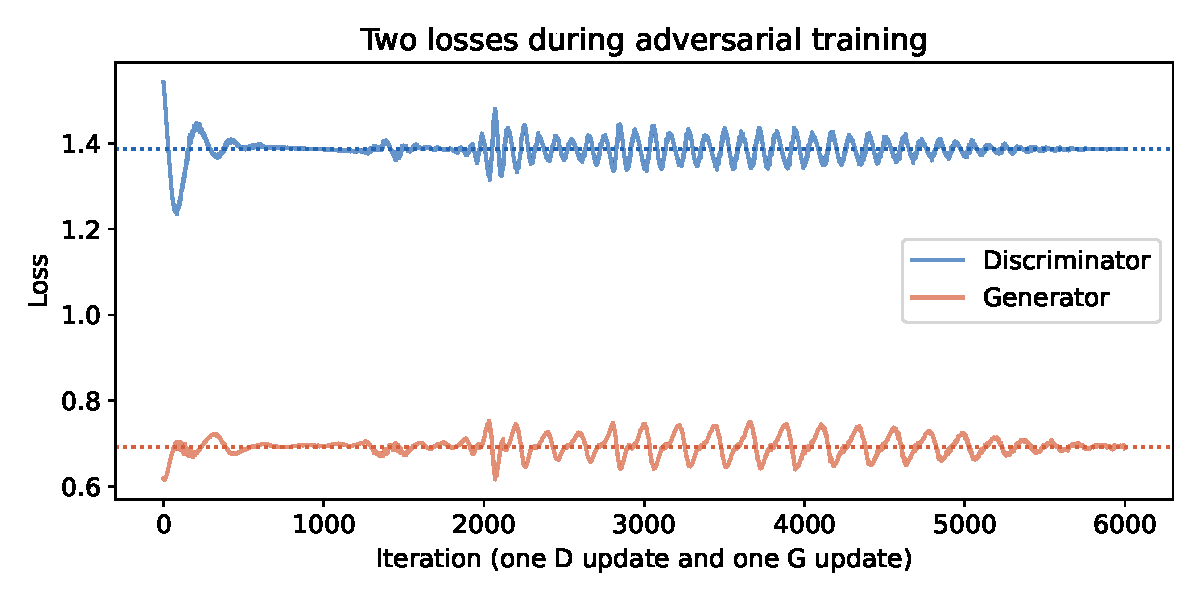
\includegraphics[width=.82\textwidth,height=.65\textheight,keepaspectratio]{figures/loss_curve.pdf}
\end{center}
\small
At $d=1/2$, our scaling gives $L_D=2\log2\approx1.386$ and $L_G=\log2\approx0.693$.\\[2mm]
The dotted lines are reference levels. A weak discriminator can reach them with poor samples.
\end{frame}

\begin{frame}[fragile]{5. Generation needs only the generator}
\begin{lstlisting}
torch.manual_seed(2026)
G.eval()
with torch.no_grad():
    real_test = 2 + 0.5 * torch.randn(5000, 1)
    generated = G(torch.randn(5000, 1))
\end{lstlisting}
\vspace{3mm}
These real samples and noise inputs are new, created after training.\\[3mm]
Compare the distributions. The first generated sample has no required match with the first real sample.\\[3mm]
\texttt{no\_grad()} is appropriate now: we are evaluating fixed parameters.
\end{frame}

\begin{frame}{Generated values before and after training}
\begin{center}
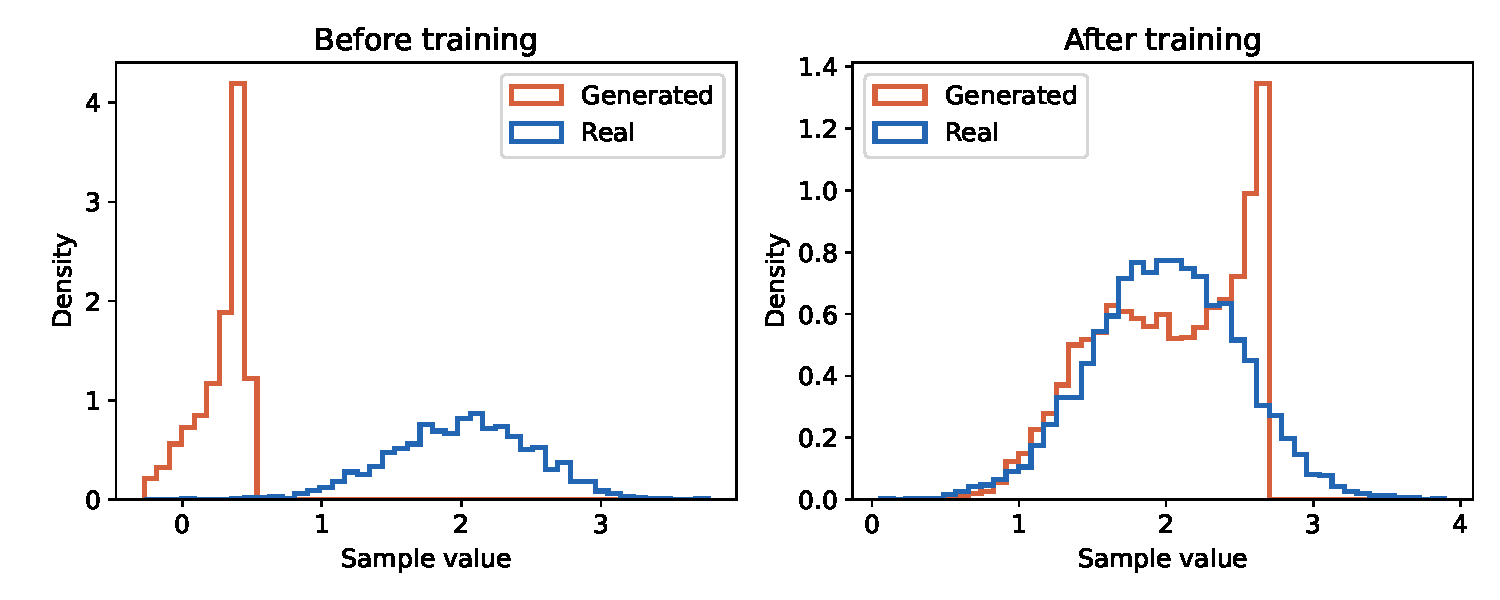
\includegraphics[width=\textwidth,height=.67\textheight,keepaspectratio]{figures/generated_distribution.pdf}
\end{center}
\small
Before: training data and the initial generator. After: fresh real and generated samples.\\[2mm]
Each histogram has total area 1. The panels use different vertical scales.
\end{frame}

\begin{frame}{Numerical checks on 5,000 new samples}
\begin{center}
\small\begin{tabular}{lrrr}
\toprule
Statistic & Target & Real test & Generated\\
\midrule
Mean & 2.00000 & 1.99510 & 2.00007\\[1.5mm]
Standard deviation & 0.50000 & 0.50366 & 0.49586\\[1.5mm]
10th percentile & 1.35922 & 1.34386 & 1.31459\\[1.5mm]
Median & 2.00000 & 2.00074 & 2.02866\\[1.5mm]
90th percentile & 2.64078 & 2.62757 & 2.63094\\[1.5mm]
\bottomrule
\end{tabular}

\end{center}
\vspace{4mm}
The table compares the theoretical target with two finite sample sets.\\[3mm]
Mean and standard deviation describe location and spread. Percentiles examine more of the shape.\\[3mm]
\small Values come from the executed notebook and round to five decimal places.
\end{frame}

\begin{frame}{Quantiles reveal differences in shape}
\begin{columns}[c]
\begin{column}{.56\textwidth}
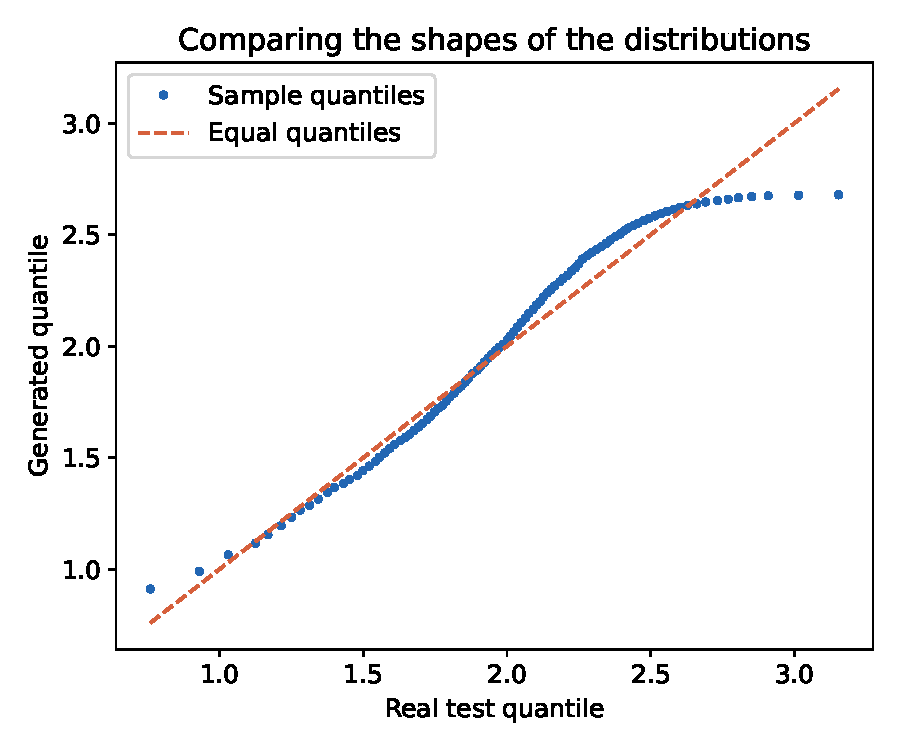
\includegraphics[width=\linewidth,height=.71\textheight,keepaspectratio]{figures/quantile_comparison.pdf}
\end{column}
\begin{column}{.40\textwidth}
\small
We compare the 1st through 99th percentiles.\\[4mm]
Near the diagonal: similar quantiles.\\[4mm]
This run flattens in the upper tail. The histogram also has excess mass near 2.7.\\[4mm]
A finite sum of \texttt{Tanh} terms is bounded. It cannot exactly reproduce an unbounded normal distribution.
\end{column}
\end{columns}
\end{frame}

\begin{frame}{The next step: generating time series}
\large
\[G_\theta(z)=(X_{t_1},X_{t_2},\ldots,X_{t_T})\]
\normalsize
\begin{itemize}\setlength\itemsep{4mm}
\item Today's generator outputs one number. A time series generator outputs an entire path or sequence.
\item Matching a histogram alone cannot establish temporal dependence.
\item Our project will investigate how Volterra signatures can contribute to generation or evaluation.
\end{itemize}
\vspace{4mm}
That method is future work. This example establishes the GAN training pattern.
\end{frame}

\begin{frame}{Experiments and discussion}
\begin{enumerate}\setlength\itemsep{3mm}
\item Change the seed. Does the same schedule give similar samples?
\item Use 1,000 iterations. Compare the losses and the histogram.
\item Use 4 hidden neurons. Does the generated spread change?
\item Try two separated peaks. Does the generator cover both?
\end{enumerate}
\vspace{4mm}
Too little variety is \alert{mode collapse}. Report unsuccessful runs too.\\[2mm]
Restart the kernel for each experiment. Use fresh test data after tuning.
\vfill
\tiny References: \href{https://arxiv.org/abs/1406.2661}{Goodfellow et al. (2014)};
PyTorch \href{https://docs.pytorch.org/tutorials/beginner/dcgan_faces_tutorial.html}{DCGAN tutorial} and
\href{https://docs.pytorch.org/docs/stable/generated/torch.nn.BCEWithLogitsLoss.html}{BCEWithLogitsLoss}.\\[2mm]
\small Companion notebook: \texttt{learning\_gans.ipynb}
\end{frame}

\end{document}
